%%%%%%%%%%%%%%%%%%%%%%%%%%%%%%%%%%%%%%%%%%%%%%%%%%%%%%%%%%%%%%%%%%%%%%%%%%%%%%%%
%2345678901234567890123456789012345678901234567890123456789012345678901234567890
%        1         2         3         4         5         6         7         8

\documentclass[letterpaper, 10 pt, conference]{ieeeconf}  % Comment this line out
                                                          % if you need a4paper
%\documentclass[a4paper, 10pt, conference]{ieeeconf}      % Use this line for a4
                                        % paper
\usepackage{graphicx}
\usepackage{amssymb}
\usepackage{amsmath}
\usepackage{breqn}
\IEEEoverridecommandlockouts                              % This command is only
                                                          % needed if you want to
                                                          % use the \thanks command
\overrideIEEEmargins
% See the \addtolength command later in the file to balance the column lengths
% on the last page of the document



% The following packages can be found on http:\\www.ctan.org
%\usepackage{graphics} % for pdf, bitmapped graphics files
%\usepackage{epsfig} % for postscript graphics files
%\usepackage{mathptmx} % assumes new font selection scheme installed
%\usepackage{times} % assumes new font selection scheme installed
%\usepackage{amsmath} % assumes amsmath package installed
%\usepackage{amssymb}  % assumes amsmath package installed

\title{\LARGE \bf
Ley de la Reflexi\'on de Ondas y la condici\'on de reflexi\'on total interna
}

%\author{ \parbox{3 in}{\centering Huibert Kwakernaak*
%         \thanks{*Use the $\backslash$thanks command to put information here}\\
%         Faculty of Electrical Engineering, Mathematics and Computer Science\\
%         University of Twente\\
%         7500 AE Enschede, The Netherlands\\
%         {\tt\small h.kwakernaak@autsubmit.com}}
%         \hspace*{ 0.5 in}
%         \parbox{3 in}{ \centering Pradeep Misra**
%         \thanks{**The footnote marks may be inserted manually}\\
%        Department of Electrical Engineering \\
%         Wright State University\\
%         Dayton, OH 45435, USA\\
%         {\tt\small pmisra@cs.wright.edu}}
%}

\author{Cesar J. Munoz Martinez$^{1}$% <-this % stops a space
\thanks{Este trabajo es realizado para la tarea 2 del curso de \'optica integrada}% <-this % stops a space
\thanks{$^{1}$Unidad de Postgrado de la Facultad de Ingenieria Electrica y electronica,
        Universidad Nacional de Ingenieria}%
}


\begin{document}



\maketitle
\thispagestyle{empty}
\pagestyle{empty}


%%%%%%%%%%%%%%%%%%%%%%%%%%%%%%%%%%%%%%%%%%%%%%%%%%%%%%%%%%%%%%%%%%%%%%%%%%%%%%%%
\begin{abstract}

Esta publicaci\'on discute los temas relacionados a la ley de la reflexi\'on de ondas para superficies con diferentes valores de indice de refracci\'on. Partiendo de la ley de Snell como principio minimo de conservacion del momentum hasta la condicion que se debe tomar en cuenta para que haya una total reflexi\'on interna.

\end{abstract}


%%%%%%%%%%%%%%%%%%%%%%%%%%%%%%%%%%%%%%%%%%%%%%%%%%%%%%%%%%%%%%%%%%%%%%%%%%%%%%%%
\section{LA LEY DE LA REFLEXI\'ON}

La f\'isica de la ley de la reflexi\'on obedece en su principio a reglas geom\'etricas, que permiten describir de mejor manera el comportamiento de las ondas de luz cuando estas atraviesan de un medio a otro, tomando en cuenta que estas medios poseen diferente de indice de refracci\'on. La Figura~\ref{fig:PrincipiGeometricoMinD}, muestra el principio de reflexi\'on de una onda de luz incidente sobre una superficie diel\'ectrica o un espejo, el cual es totalmente reflejado sim\'etricamente respecto a la recta normal a la superficie del espejo, con el mismo \'angulo. La ruta seguida por el rayo incidente partiendo desde el punto P, se demuestra que al llegar a la ruta P', este recorrido la ruta de m\'inima longitud posible para llegar a su destino. Esto es facilmente demostrable mediante adecuaciones geom\'etricas, dado que al reflejar sim\'etricamente P' en P'' se observa que la l\'inea recta P'OP" es siempre menor que la suma de los lados del triagulo formado por el tercer punto de incidencia hipot\'etico de la luz en caso no cumpliese esta regla de ruta de recorrido m\'inimo.
% +++Figura 1+++
\begin{figure}[ht!]
\centering{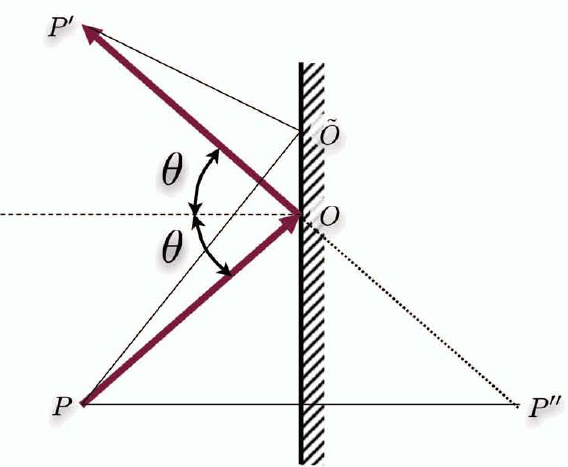
\includegraphics[width=80mm]{imagenes/PrincipiGeometricoMinD.png}}
\caption{Ley de Reflexi\'on sim\'etrico de un modelo de rayos. Fuente:~\cite{1}
}\label{fig:PrincipiGeometricoMinD}
\end{figure}
La Figura~\ref{fig:PrincipiGeometrico2} muestra la reflexi\'on en espejos, como se puede observar esta reflexi\'on es producida como si esta estubiese recorriendo una ruta lineal directa desde un punto proyectado sim\'etricamente tomando al espejo como plano de simetr\'ia.

% +++Figura 2+++
\begin{figure}[ht!]
\centering{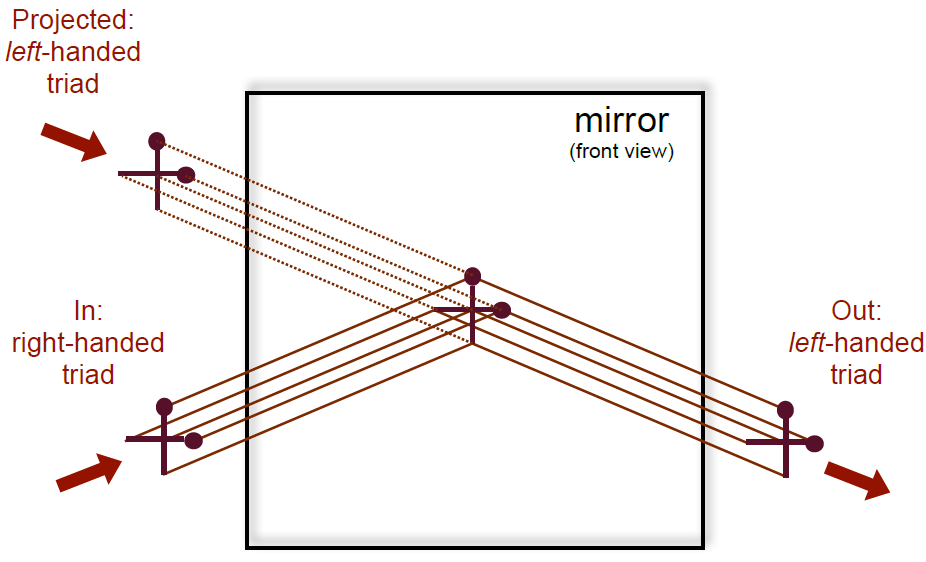
\includegraphics[width=80mm]{imagenes/PrincipioReflexion2.png}}
\caption{Ley de Reflexi\'on sim\'etrico de un modelo de rayos. Fuente:~\cite{1}
}\label{fig:PrincipiGeometrico2}
\end{figure}

\section{LEY DE LA REFRACCI\'ON}

\subsection{Deduccion de la ley de Snell}
La trayectoria seguida un por un rayo refractado desde P a P', segun el principio de Fermat, el angulo\(\theta\), debe ser tal que la ruta PP' deba ser la mas m\'inima posible.
% +++Figura 3+++
\begin{figure}[ht!]
\centering{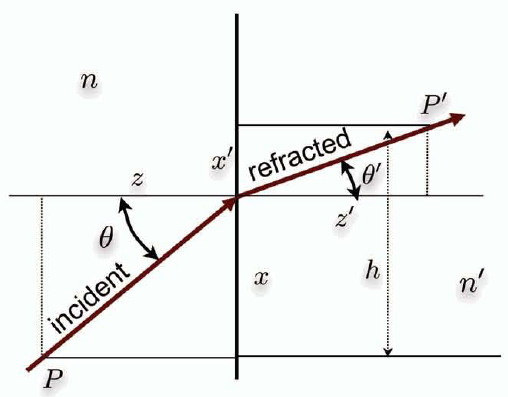
\includegraphics[width=80mm]{imagenes/PrincipioRefraccion.png}}
\caption{Ley de Refracci\'on de un modelo de rayos. Fuente:~\cite{1}
}\label{fig:PrincipioRefraccion}
\end{figure}
Esta Longitud de ruta es expresada mediante la ecuacion~\eqref{eq:rutaminimaOPL}. 

\begin{equation}
\label{eq:rutaminimaOPL}
{
(OPL) = n\sqrt {{x^2} + {z^2}}  + {n^'}\sqrt {{{(h - x)}^2} + {z^{'2}}}
}
\end{equation}
Para obtener el valor minimo de la ruta tomando en cuenta la variacion respecto a x, derivamos la ecuacion~\eqref{eq:rutaminimaOPL}, resultando la ecuacion~\eqref{eq:minimadistanciarefr}.
\begin{equation}
\label{eq:minimadistanciarefr}
{
\frac{{\partial (OPL)}}{{\partial x}} = n\frac{x}{{\sqrt {{x^2} + {z^2}} }} - {n^'}\frac{{h - x}}{{\sqrt {{{(h - x)}^2} + {z^{'2}}} }}
}
\end{equation}
Para obtener el valor un minimo relativo se iguala la ecuacion~\eqref{eq:minimadistanciarefr} a cero. El cual resulta en la ley de Snell, descrito por la ecuacion~\eqref{eq:leySnell}.
\begin{equation}
\label{eq:leySnell}
{
n\sin \theta  - {n^'}\sin {\theta ^'} = 0 \to n\sin \theta  = {n^'}\sin {\theta ^'}
}
\end{equation}
\subsection{Ley de Snell como principio de la conservacion del momentum}
La Figura~\ref{fig:PrincipioConservacionMomentumSnell}, muestra la representacion en esferas de descartes, del momentum representado en un medio determinado con un radio igual un indice de refraccion n menor al medio con indice de refraccion n'. Debido  que se considera una superficie lisa, se considera conservacion del momentum lineal lateral al eje optico, mientras debido al cambio del medio el momentum longitudinal paralelo al eje optico varia.

% +++Figura 4+++
\begin{figure}[ht!]
\centering{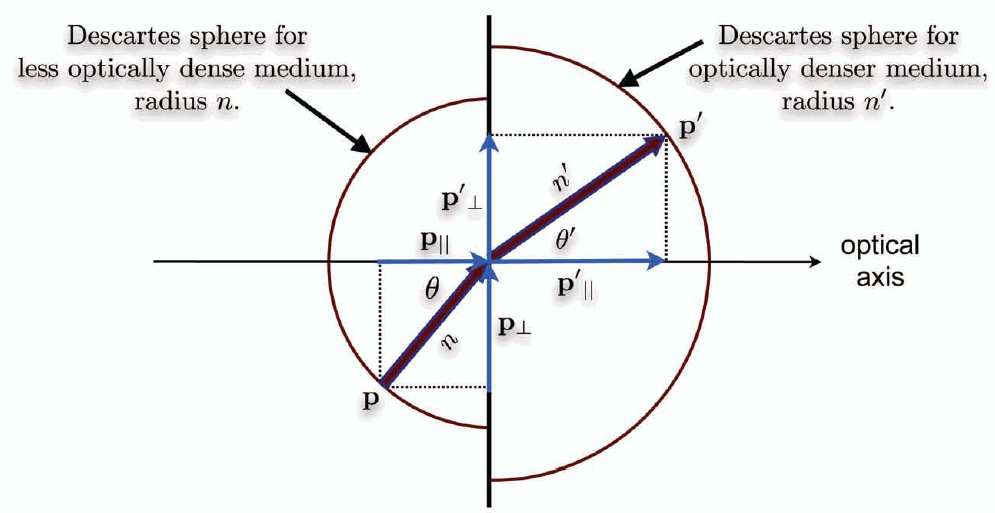
\includegraphics[width=80mm]{imagenes/PrincipioConservacionMomentumSnell.png}}
\caption{Conservacion del momentum para la ley de Snell. Fuente:~\cite{1}
}\label{fig:PrincipioConservacionMomentumSnell}
\end{figure}
Las Ecuaciones ~\eqref{eq:cantidadmovimientolong} y~\eqref{eq:cantidadmovimientolat}, explican matematicamente este comportamiento fisico.
\begin{equation}
\label{eq:cantidadmovimientolong}
{
p|| \ne {p^'}||
}
\end{equation}

\begin{equation}
\label{eq:cantidadmovimientolat}
{
p \bot  = {p^'} \bot
}
\end{equation}
En la Figura~\ref{fig:TiposRefraccion}, se muestra los dos casos de refraccion que puede ocurrir, cuando el rayo va desde una superficie de menor indice de refraccion a una de mayor indice de refraccion y la segunda es el caso viceversa, de un medio de mayor indice de refraccion a uno de menor indice de refraccion.
% +++Figura 5+++
\begin{figure}[ht!]
\centering{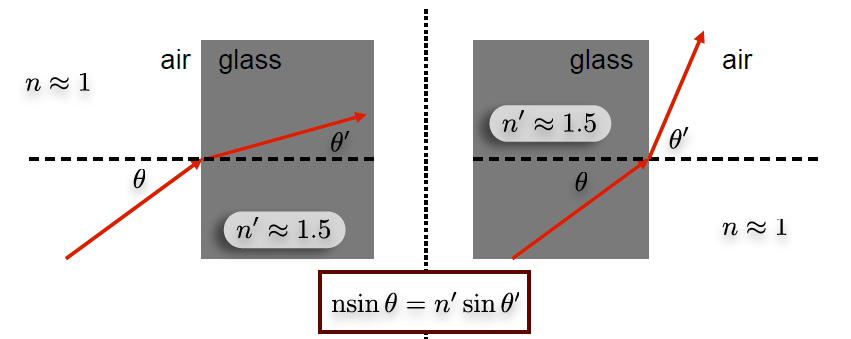
\includegraphics[width=80mm]{imagenes/TiposRefraccion.png}}
\caption{Conservacion del momentum para la ley de Snell. Fuente:~\cite{1}
}\label{fig:TiposRefraccion}
\end{figure}
En el primer caso, se observa que al pasar del medio de menor indice de refraccion la ley de snell puede ser satisfecho incluso si el angulo de refraccion es lo suficientemente bajo para un angulo de indicidencia maxima. Esta conclusion podria describirse mediante la ecuacion~\eqref{eq:ecuacioncaso1refraccion}.
\begin{equation}
\label{eq:ecuacioncaso1refraccion}
{
{n^'}\sin {\theta ^'} = n
}
\end{equation}
En el segundo caso, no necesariamente la ley de snell puede ser satisecha debido a  que si para un angulo de indicidencia dado se presenta lo descrito en la ecuacion~\eqref{eq:ecuacioncaso2refraccion} , entonces se presenta una situacion muy aprovechada en la ingenieria de las comunicaciones opticas, lo que se conoce como el escenario de la total reflexion interna, en el cual el rayo incidente es totalmente reflejado y no hay rayo refractado.
\begin{equation}
\label{eq:ecuacioncaso2refraccion}
{
{n^'}\sin \theta  > n
}
\end{equation}
\section{PRINCIPIO DE LA REFLEXION TOTAL INTERNA}
La Figura~\ref{fig:TIR}, muestra el caso de la situacion antes mencionada, el principio de reflexion total interna, en el caso en el cual si la ecuacion~\eqref{eq:ecuacioncasoangulocritico} es satisfecha el angulo incidente del medio mas denso opticamente, es llamado angulo critico. Para valores mayor que el se producira total reflexion interna en el medio optico mas denso y no cumplira la ley de refraccion de snell. Se observa tambien que para un angulo critico, la luz refractada se propaga paralelo a la interfaz del cambio de medio, lo que resulta ondas superficiales que decaen a medida que se aleja del medio mas denso. Este ondas tambien se encuentran presentes en la reflexion total interna y son conocidas como ondas evanescentes. En la Figura~\ref{fig:TIR} se puede observa el decaimiento del campo electrico evanescente de manera exponencial.
\begin{equation}
\label{eq:ecuacioncasoangulocritico}
{
{n_c}\sin {\theta _c} = 1
}
\end{equation}


% +++Figura 6+++
\begin{figure}[ht!]
\centering{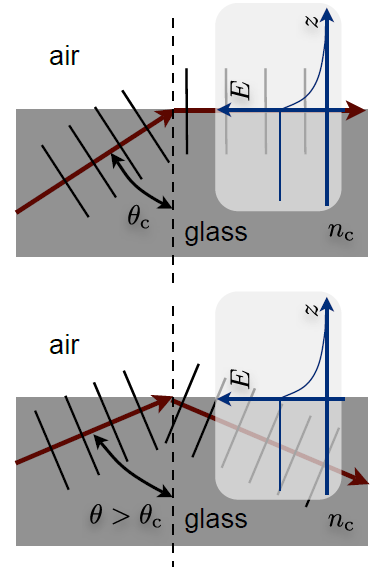
\includegraphics[width=60mm]{imagenes/TIR.png}}
\caption{Total reflexion interna. Fuente:~\cite{1}
}\label{fig:TIR}
\end{figure}

\begin{thebibliography}{}

\bibitem{1}
National University of Singapur, MiT.: `The law of reflection, lecturer',
\textit{MiT Lecturer}, 2008

\end{thebibliography}
\end{document}
